% Editable vector schematic; included inside the poster's first figure.
% Left: physical plant. Right: the two switching curves from the paper.
\begin{tikzpicture}[x=1cm,y=1cm,
  labeltext/.style={font=\small,text=ink,align=center},
  arrow/.style={-{Stealth[length=4mm]},very thick,draw=accent}]
\useasboundingbox (0,-5.0) rectangle (38,11.2);
\fill[accent!4,rounded corners=3mm] (0,0) rectangle (11.5,11.2);
\node[labeltext,font=\small\bfseries] at (5.75,10.35) {Muscle-driven elbow};
% Upper arm, elbow and forearm: schematic only, not anatomical geometry.
\draw[ink,line width=4mm,line cap=round] (4.2,8.2)--(4.2,4.1)--(8.5,1.6);
\draw[white,line width=1.4mm,line cap=round] (4.2,8.2)--(4.2,4.1)--(8.5,1.6);
\filldraw[fill=white,draw=ink,line width=1.2mm] (4.2,4.1) circle (.38);
\draw[accent,line width=2.5mm,line cap=round] (3.8,7.5)..controls (1.4,5.6) and (3.5,4.0)..(5.65,3.25);
\draw[ink,dashed] (4.2,4.1)--(4.2,1.0);
\draw[arrow] (4.2,2.5) arc[start angle=270,end angle=330,radius=1.6];
\node[labeltext] at (5.6,1.1) {$\theta$};
\node[labeltext,anchor=east] at (3.0,6.1) {$a$};
\node[labeltext] at (7.8,7.9) {brachialis};
\draw[ink] (7.4,7.2)--(4.2,6.0);
\draw[arrow] (8.1,3.9)--(8.1,2.2);
\node[labeltext,anchor=west] at (8.25,3.4) {$mg$};
\node[labeltext] at (5.75,.35) {$\theta^\ast=60^\circ,\quad a^\ast=0.113$};

\node[labeltext,font=\small\bfseries] at (25.0,10.35) {Two switches at the same equilibrium};
\node[anchor=center,inner sep=0] at (25.0,5.1)
  {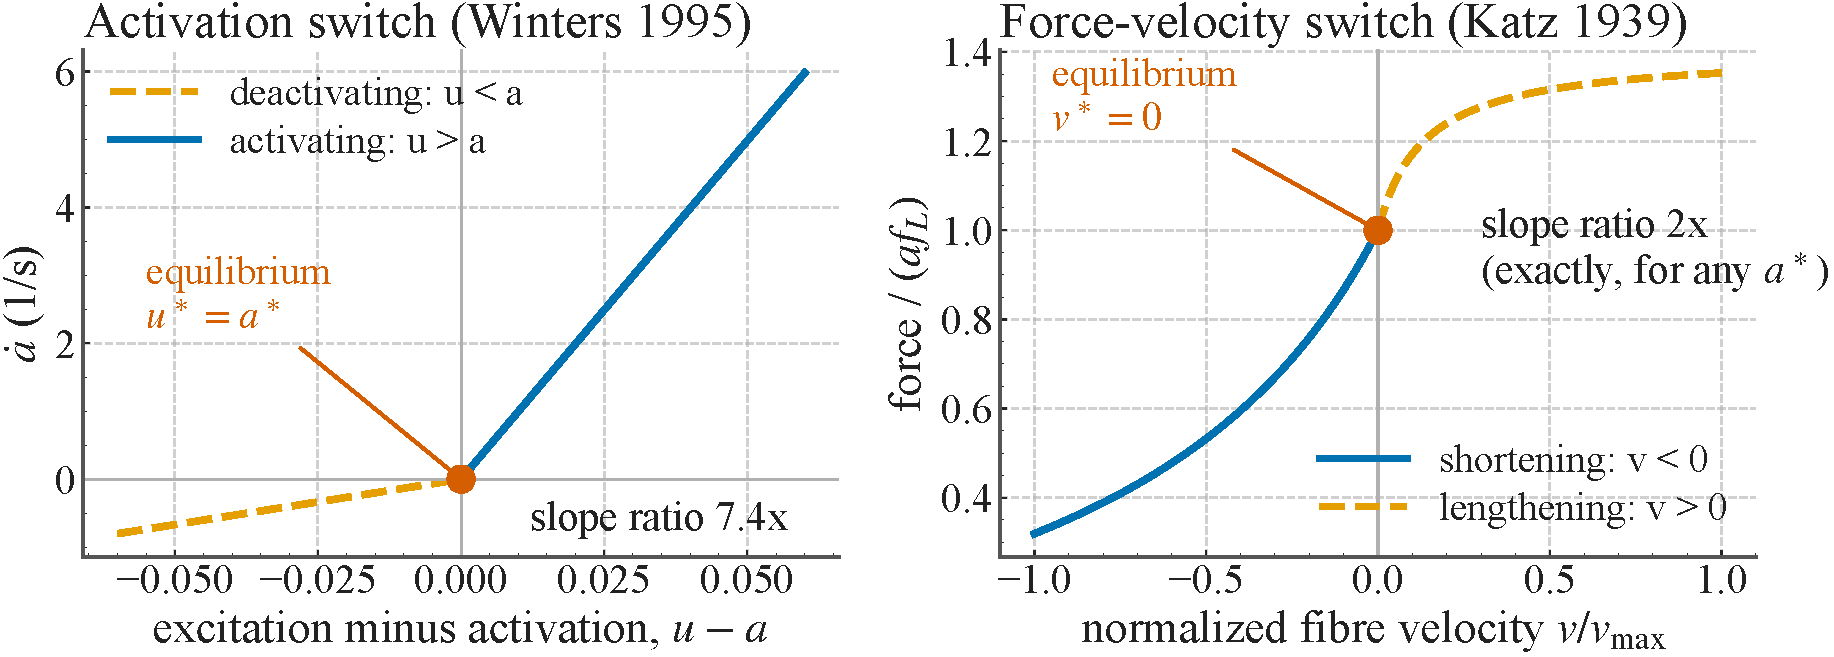
\includegraphics[width=25cm]{fig1_kinks.pdf}};


% The perturbation signs select the directional Jacobian.
\node[draw=accent,fill=accent!5,rounded corners=2mm,labeltext,
  text width=16.5cm,minimum height=3.8cm] (modes) at (9,-2.65)
  {\textbf{Four directional models}\\[.3ex]
  $\{u-a>0,\ u-a\le0\}\ \times\ \{v>0,\ v\le0\}$\\[.3ex]
  $\delta\dot x=A_i\delta x+B_i\delta u$};
\node[draw=accent,fill=accent!5,rounded corners=2mm,labeltext,
  text width=15.3cm,minimum height=3.8cm] (mpc) at (29.6,-2.65)
  {\textbf{Update the prediction model}\\[.3ex]
   Measured state $\to$ active branch $\to$ MPC\\[.3ex]
   Test prediction and tracking transients};
\draw[arrow] (modes.east)--(mpc.west);
\end{tikzpicture}
